% $Id: Attribute_obj.tex,v 1.16 2011/01/05 20:05:41 svasquez Exp $
%
% Earth System Modeling Framework
% Copyright 2002-2011, University Corporation for Atmospheric Research,
% Massachusetts Institute of Technology, Geophysical Fluid Dynamics
% Laboratory, University of Michigan, National Centers for Environmental
% Prediction, Los Alamos National Laboratory, Argonne National Laboratory,
% NASA Goddard Space Flight Center.
% Licensed under the University of Illinois-NCSA License.

Each Attribute contains a name-value pair in which the value can be any of several numeric, character, and logical types.  The available ESMF Attribute value types include:

\label{table:attTypes}
\begin{itemize}
\item {\tt ESMF\_TYPEKIND\_I4}
\item {\tt ESMF\_TYPEKIND\_I4} list
\item {\tt ESMF\_TYPEKIND\_I8}
\item {\tt ESMF\_TYPEKIND\_I8} list
\item {\tt ESMF\_TYPEKIND\_R4}
\item {\tt ESMF\_TYPEKIND\_R4} list
\item {\tt ESMF\_TYPEKIND\_R8}
\item {\tt ESMF\_TYPEKIND\_R8} list
\item {\tt ESMF\_TYPEKIND\_Logical}
\item {\tt ESMF\_TYPEKIND\_Logical} list
\item {\tt EMSF\_TYPEKIND\_Character}
\item {\tt EMSF\_TYPEKIND\_Character} list
\end{itemize}

The other members of the Attribute class can be seen in Figure \ref{fig:AttributeClassUML}  below, which shows a UML representation of the ESMF Attribute class.

In addition to a name, all Attributes within an Attribute package are identified by a convention, purpose, and the ESMF object type they are associated with. These are additional strings that are initialized as empty until specified. 

Also, all Attributes contain three vectors of pointers to other Attributes, which are empty until specified otherwise.  These vectors of Attribute pointers hold the Attributes, Attribute packages, and Attribute links.  This feature is what allows the Attribute class to self assemble complex structures for representing and organizing the metadata of an ESMF object hierarchy.

For a more detailed view of how Attribute packages and hierarchies are formed, see Figures \ref{fig:AttributePackageUML} and \ref{fig:AttributeHierarchyUML}, respectively.

\begin{figure}[h]
\centering
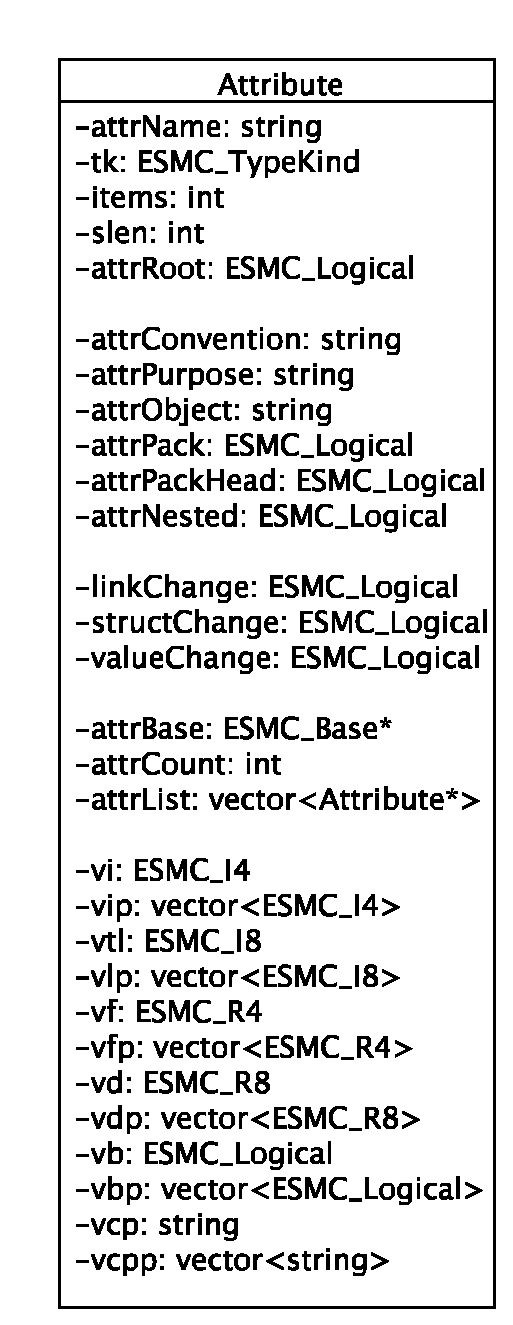
\includegraphics{AttributeClassUML}
\caption{The structure of the Attribute class}
\label{fig:AttributeClassUML}
\end{figure}
\clearpage

\begin{figure}[h]
\centering
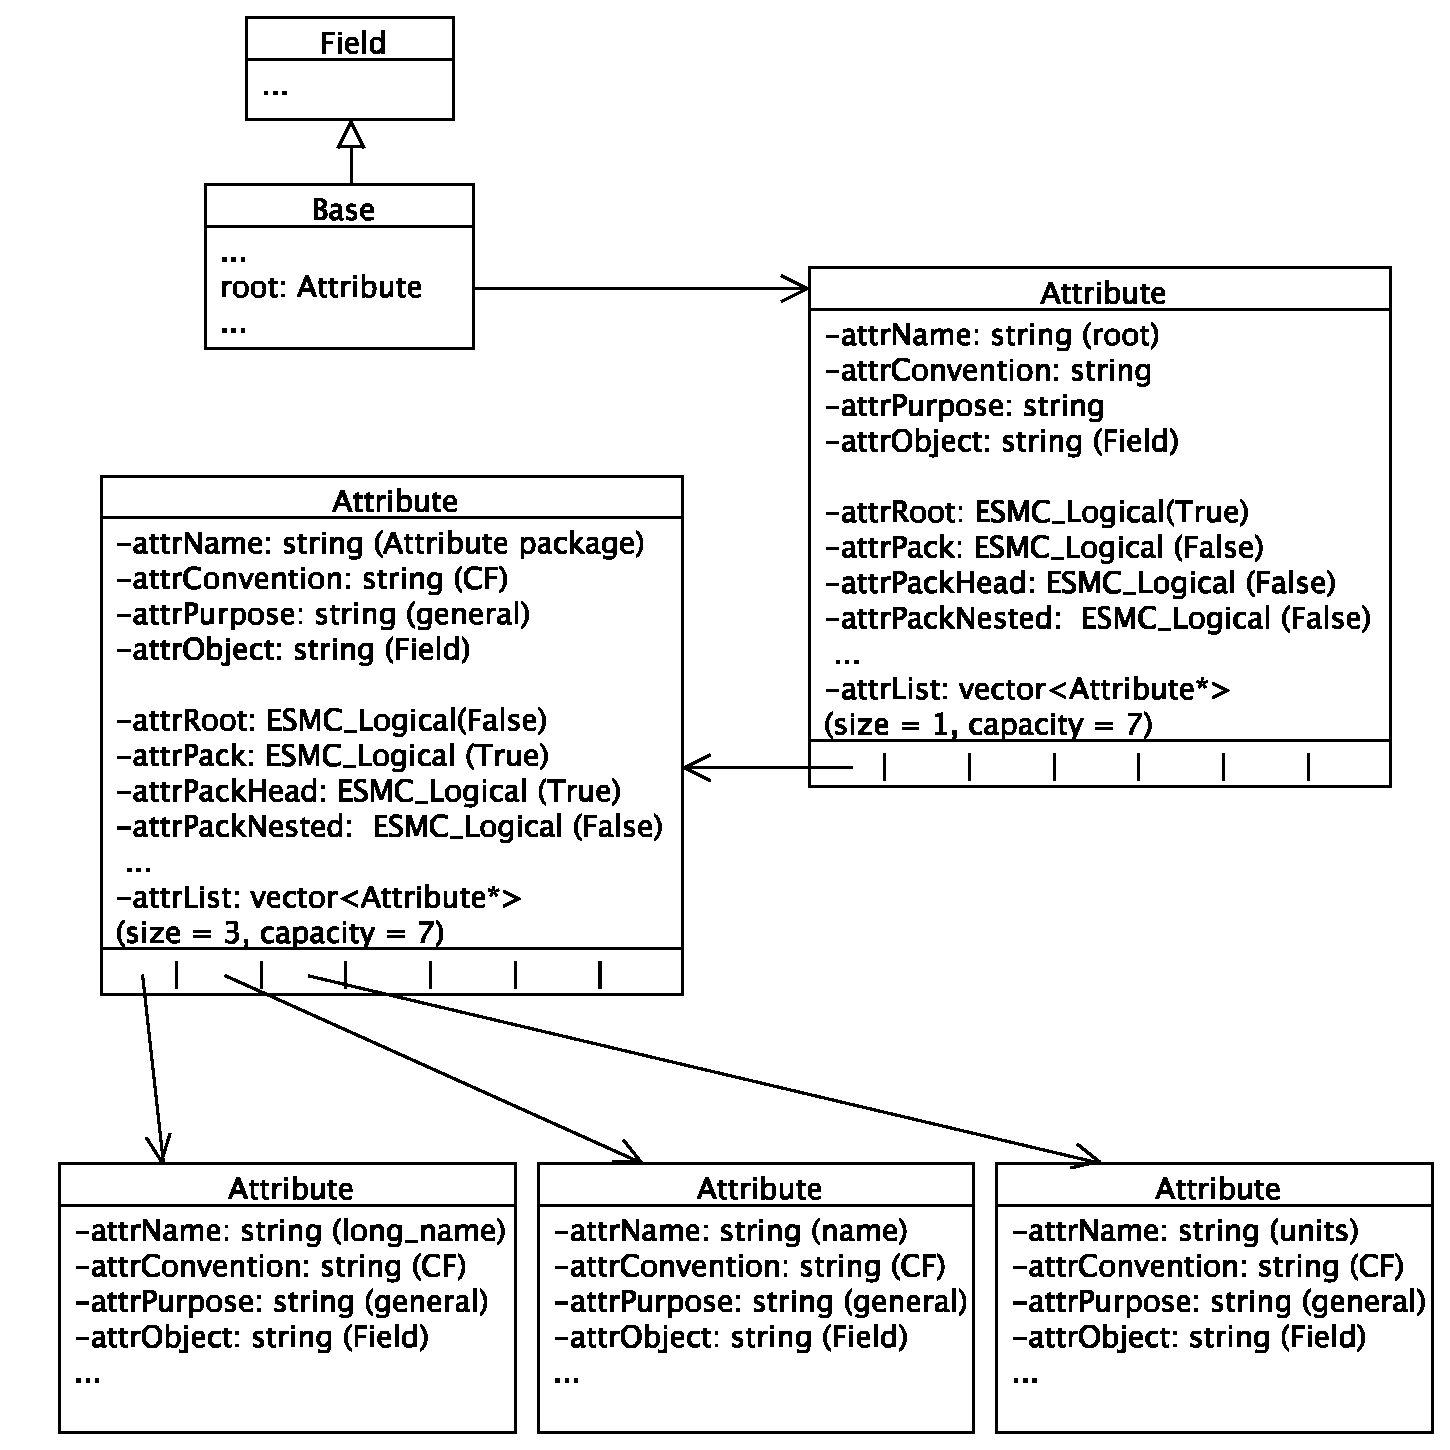
\includegraphics[width=5.5in,height=6in]{AttributePackageUML}
\caption{The internal object organization for the representation of Attribute packages}
\label{fig:AttributePackageUML}
\end{figure}
\clearpage

\begin{figure}[h]
\centering
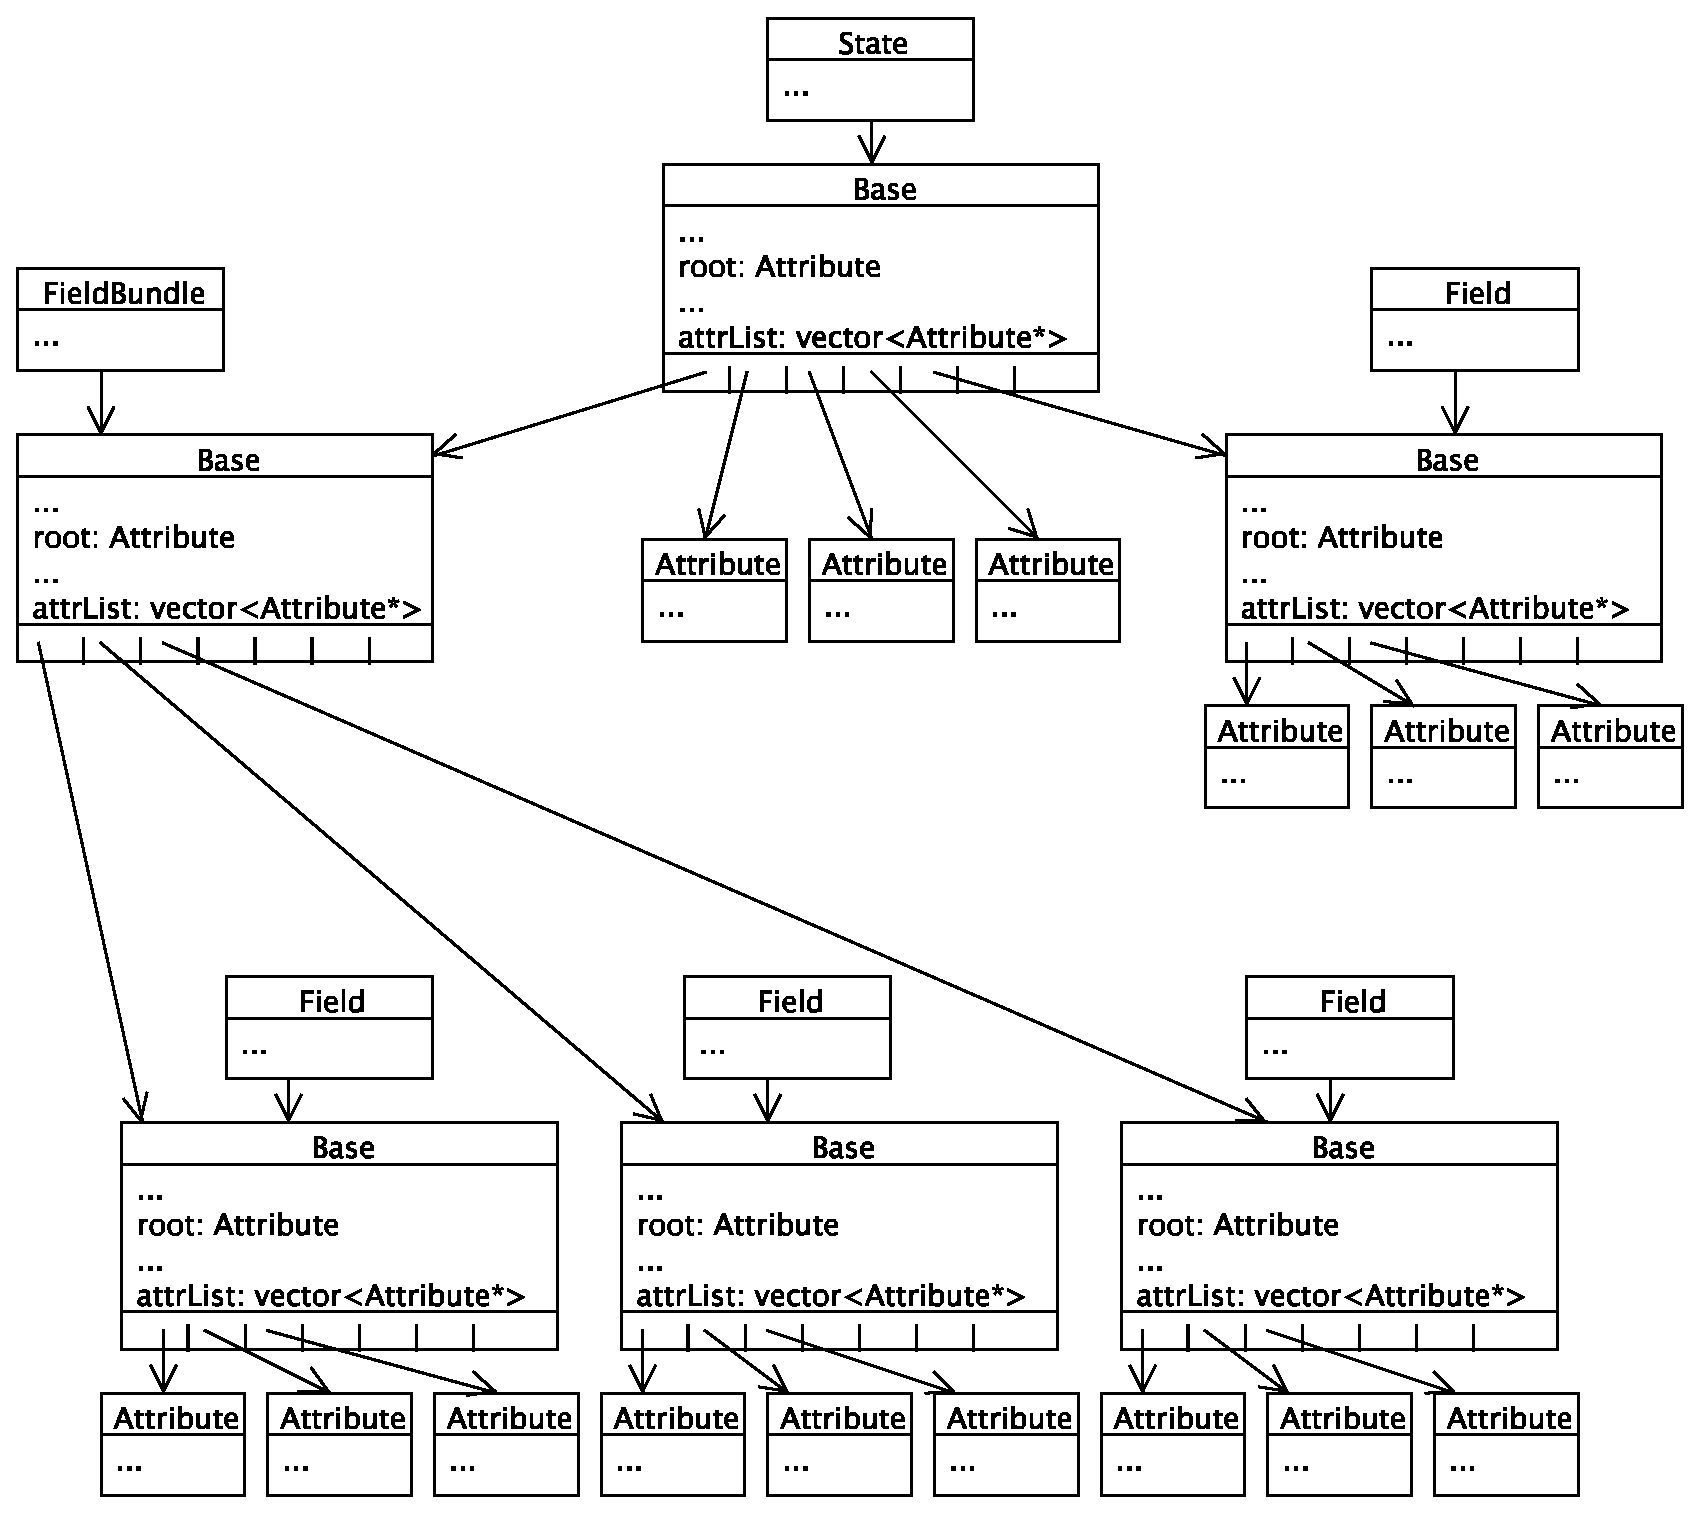
\includegraphics[width=5.5in,height=6in]{AttributeHierarchyUML}
\caption{The internal object organization for the representation of Attribute hierarchies}
\label{fig:AttributeHierarchyUML}
\end{figure}
\clearpage
